%%%%%%%%%%%%%%%%%%%%%%%%%%%%%%%%%%%%%%%%%
% Beamer Presentation
% LaTeX Template
% Version 1.0 (10/11/12)
%
% This template has been downloaded from:
% http://www.LaTeXTemplates.com
%
% License:
% CC BY-NC-SA 3.0 (http://creativecommons.org/licenses/by-nc-sa/3.0/)
%
%%%%%%%%%%%%%%%%%%%%%%%%%%%%%%%%%%%%%%%%%

% References:
%  - https://en.wikibooks.org/wiki/LaTeX/Presentations (wikibooks beamer manual)
%  - http://texdoc.net/texmf-dist/doc/latex/beamer/doc/beameruserguide.pdf (beamer manual -- official guide)
%  - https://www.latex-project.org/publications/fmittelbach-1a-2017.pdf (sample beamer presentation)

%----------------------------------------------------------------------------------------
%	PACKAGES AND THEMES
%----------------------------------------------------------------------------------------

% TODO(tperrotta): add the final option once the slides are complete
% [handout]
% \documentclass[12pt,final]{beamer}
\documentclass[12pt]{beamer}

\mode<presentation> {

% The Beamer class comes with a number of default slide themes
% which change the colors and layouts of slides. Below this is a list
% of all the themes, uncomment each in turn to see what they look like.

% reference and preview: http://deic.uab.es/~iblanes/beamer_gallery/index_by_theme_and_color.html (sample themes and colors)

%\usetheme{default}
%\usetheme{AnnArbor}
%\usetheme{Antibes}
%\usetheme{Bergen}
%\usetheme{Berkeley}
%\usetheme{Berlin}
%\usetheme{Boadilla}
%\usetheme{CambridgeUS}
%\usetheme{Copenhagen}
%\usetheme{Darmstadt}
%\usetheme{Dresden}
\usetheme{Frankfurt}
%\usetheme{Goettingen}
%\usetheme{Hannover}
%\usetheme{Ilmenau}
%\usetheme{JuanLesPins}
%\usetheme{Luebeck}
%\usetheme{Madrid}
%\usetheme{Malmoe}
%\usetheme{Marburg}
%\usetheme{Montpellier}
%\usetheme{PaloAlto}
%\usetheme{Pittsburgh}
%\usetheme{Rochester}
%\usetheme{Singapore}
%\usetheme{Szeged}
%\usetheme{Warsaw}

% As well as themes, the Beamer class has a number of color themes
% for any slide theme. Uncomment each of these in turn to see how it
% changes the colors of your current slide theme.

%\usecolortheme{albatross}
\usecolortheme{beaver}
%\usecolortheme{beetle}
%\usecolortheme{crane}
%\usecolortheme{dolphin}
%\usecolortheme{dove}
%\usecolortheme{fly}
%\usecolortheme{lily}
%\usecolortheme{orchid}
%\usecolortheme{rose}
%\usecolortheme{seagull}
%\usecolortheme{seahorse}
%\usecolortheme{whale}
%\usecolortheme{wolverine}

%\setbeamertemplate{footline} % To remove the footer line in all slides uncomment this line
\setbeamertemplate{footline}[page number] % To replace the footer line in all slides with a simple slide count uncomment this line

%\setbeamertemplate{navigation symbols}{} % To remove the navigation symbols from the bottom of all slides uncomment this line
\beamertemplatenavigationsymbolsempty

% grey out items after pause
\setbeamercovered{transparent,highly dynamic}

% reduce spacing between figure/table and captions
% https://tex.stackexchange.com/questions/226127/how-to-remove-spacing-between-figure-and-caption-in-the-beamer-class
% \setlength\abovecaptionskip{-5pt}

\setbeamertemplate{itemize items}[default]
\setbeamertemplate{enumerate items}[default]
}

\usepackage{iftex}
\ifPDFTeX
  % use UTF-8 in pdftex (not needed in LuaTeX and XeTeX)
  \usepackage[utf8]{inputenc}
\fi

% document language (the latest option is set as the current active language)
\usepackage[english,portuguese]{babel}

% math and symbols
\usepackage{amsmath,amssymb}

% next-generation computer modern fonts
\usepackage{lmodern}

% Allows including images
\usepackage{graphicx}

% required for better tables
\usepackage{longtable}
\usepackage{multirow}
\usepackage{makecell}

% curly brackets besides tables (\ldelim, \rdelim)
\usepackage{bigdelim}

\usepackage[font=small]{caption}

% Allows the use of \toprule, \midrule and \bottomrule in tables
\usepackage{booktabs}

% text highlighting, underlining, spacing
\usepackage{soul}

% todo notes
\usepackage[obeyFinal,portuguese,textsize=footnotesize]{todonotes}

% custom todo notes macros
\newcommand{\todox}[2][]{\sethlcolor{yellow}\texthl{#1}\todo[author=\textbf{TODO},inline,color=yellow]{#2}}
\newcommand{\perrotta}[2][]{\sethlcolor{pink}\texthl{#1}\todo[author=\textbf{Thiago Perrotta},inline,color=pink]{#2}}
\newcommand{\silva}[2][]{\sethlcolor{lightgray}\texthl{#1}\todo[author=\textbf{Vitor Silva},inline,color=lightgray]{#2}}

% \listoftodos{} is incompatible with beamer
% source: https://tex.stackexchange.com/questions/313426/list-of-todos-in-beamer

% speaker notes
% reference: https://gist.github.com/andrejbauer/ac361549ac2186be0cdb
\usepackage{pgfpages}
\setbeamertemplate{note page}{\pagecolor{yellow!5}\insertnote}
%\setbeamertemplate{note page}[plain]

% These slides also contain speaker notes. You can print just the slides, just the notes, or both, depending on the setting below. Comment out the one you want.
%\setbeameroption{hide notes} % Only slides
%\setbeameroption{show notes}
%\setbeameroption{show only notes} % Only notes
%\setbeameroption{show notes on second screen=right} % Both

\usepackage{listings}
\renewcommand{\lstlistingname}{Código}
\lstset{basicstyle=\footnotesize\sf}

\lstset{%
  aboveskip=15pt,
  belowskip=15pt,
  breakatwhitespace=false,     % sets if automatic breaks should only happen at whitespace
  breaklines=true,             % sets automatic line breaking
  postbreak=\mbox{\textcolor{red}{$\hookrightarrow$}\space},
  captionpos=t,                % sets the caption-position
  columns=fullflexible,
  commentstyle=\color{gray},   % sets the comments color
  escapechar=\%,               % write LaTeX inside listings
  frame=lines,                 % adds a frame
  numbers=left,                % where to put the line-numbers
  numberstyle=\footnotesize\color{gray}, % the size of the fonts that are used for the line-numbers (alt: \tiny)
  showspaces=false,            % show spaces adding particular underscores
  showstringspaces=false,      % underline spaces within strings
  showtabs=false,              % show tabs within strings adding particular underscores
  stepnumber=1,                % the step between two line-numbers. If it's 1 each line
  stringstyle=\color{gray},
  tabsize=2,                   % sets default tabsize to 4 spaces
  title=\lstname,              % show the filename of files included with \lstinputlisting;
}

\lstdefinelanguage{sqlresults}{%
  aboveskip=5pt,
  belowskip=5pt,
  basicstyle=\footnotesize\ttfamily,
  columns=fixed,
  numbers=none,
  frame=none,
}

% hyperlinks
\hypersetup{%
  portuguese,
  pdfencoding=auto,
  breaklinks=true,
  bookmarksopen=true,
  colorlinks=true, % false: boxed links; true: colored links
  linkcolor=, % https://tex.stackexchange.com/questions/13423/how-to-change-the-color-of-href-links-for-real
  pdfstartview={FitH}, % fits the width of the page to the window
  pdfauthor={Thiago Barroso Perrotta},
  pdfcreator={Thiago Barroso Perrotta},
  pdfproducer={Thiago Barroso Perrotta},
  pdftitle={Análise do Rastro de Proveniência em Simulações Computacionais em Larga Escala},
  pdfsubject={Análise do Rastro de Proveniência em Simulações Computacionais em Larga Escala},
  pdfkeywords={Workflows Científicos,Análise de Dados Científicos,Gerência de Fluxos de Dados,Dados de Proveniência,Bancos de Dados},
}

%----------------------------------------------------------------------------------------
%	TITLE PAGE
%----------------------------------------------------------------------------------------
\title[Análise do Rastro de Proveniência]{Análise do Rastro de Proveniência em Simulações Computacionais em Larga Escala} % The short title [] appears at the bottom of every slide, the full title is only on the title page

\author[Thiago B. Perrotta]{Thiago Barroso Perrotta} % Your name
\institute[UFRJ] % Your institution as it will appear on the bottom of every slide, may be shorthand to save space
{
Engenharia de Computação e Informação \\ \smallskip
Escola Politécnica --- Universidade Federal do Rio de Janeiro \\ % Your institution for the title page
\medskip
\href{mailto:perrotta.thiago@poli.ufrj.br}{\nolinkurl{perrotta.thiago@poli.ufrj.br}} % Your email address
}
\date{14 de Setembro de 2017} % Date, can be changed to a custom date

\pgfdeclareimage[height=1.5cm]{university-logo}{escola-politecnica-ufrj}
\logo{\pgfuseimage{university-logo}}

% https://tex.stackexchange.com/questions/44983/beamer-removing-headline-and-its-space-on-a-single-frame-for-plan-but-keepin
\makeatletter
    \newenvironment{withoutheadline}{
        \setbeamertemplate{headline}[default]
        \def\beamer@entrycode{\vspace*{-\headheight}}
    }{}
\makeatother

% https://tex.stackexchange.com/questions/53781/how-can-i-include-the-logo-in-some-slides-and-remove-in-others-using-beamer
\newcommand{\nologo}{\setbeamertemplate{logo}{}} % command to set the logo to nothing

% \includeonlyframes{
% label1,
% label2,
% }

\begin{document}

%----------------------------------------------------------------------------------------
%	PRESENTATION SLIDES
%----------------------------------------------------------------------------------------

%------------------------------------------------
% \section{Section Example} Sections can be created in order to organize your presentation into discrete blocks, all sections and subsections are automatically printed in the table of contents as an overview of the talk

% \subsection{Subsection Example} % A subsection can be created just before a set of slides with a common theme to further break down your presentation into chunks
%------------------------------------------------

%---------------------------
% SLIDES BASICS:
%---------------------------

%------------------------------------------
% \tableofcontents[currentsection,currentsubsection]
%
% \begin[fragile,label=frame1]{frame}{Title}{Subtitle}
%
% \frametitle{Title}
% \framesubtitle{Subtitle}
%
% \begin{itemize}[<+->]
% \item Item 1.
% \item Item 2.
% \begin{itemize}[<.->]
%   \item<.> Sub-Item 1.
%   \item Sub-Item 2.
% \end{itemize}
%
% \end{itemize}
%
% \begin{enumerate}
% \item Item 1.
% \item Item 2.
% \end{enumerate}
%
% \begin{block}{Block 1}
% Lorem ipsum dolor.
% \end{block}
%
% \begin{alertblock}{Block 1}
% Lorem ipsum dolor.
% \end{alertblock}
%
% \begin{exampleblock}{Block 1}
% Lorem ipsum dolor.
% \end{exampleblock}
%
% \note[item]{Note that this slide is boring.}
%
% \end{frame}
%------------------------------------------

% Print the title page as the first slide
% https://tex.stackexchange.com/questions/33767/remove-section-header-from-a-beamer-theme-singapore
{
\setbeamertemplate{headline}{}
\setbeamertemplate{footline}{}
\begin{frame}
  \titlepage{}
\end{frame}
% \frame{\titlepage}
\addtocounter{page}{-1}
}

%------------------------------------------------

% Print the table of contents
\begin{withoutheadline}
\setbeamertemplate{footline}{}
\begin{frame}{Agenda}
  \tableofcontents{} % Throughout your presentation, if you choose to use \section{} and \subsection{} commands, these will automatically be printed on this slide as an overview of your presentation
\end{frame}
\end{withoutheadline}

%------------------------------------------------

\section{Introdução}
\subsection*{}

\begin{frame}{Introdução / Motivação}
\todox{Introdução}
\end{frame}

%------------------------------------------------

\section{Referencial Teórico}
\subsection*{Referencial Teórico}

\begin{frame}[t]{Fluxo de dados}

\centerline{$D = (T, S, \Phi)$}

$\left\{
\begin{tabular}{p{\textwidth}}
\begin{itemize}
    \item \( T = \{dt_1, dt_2, \ldots, dt_{\alpha}\} \) : conjuntos de \alert{transformações}
    \item \( S = \{ds_1, ds_2, \ldots, ds_{\beta}\} \) : conjuntos de \alert{dados}
    \item \( \Phi = \{\phi_1, \phi_2, \ldots, \phi_{\gamma}\} \) : \alert{dependências} de dados
\end{itemize}
\end{tabular}
\right.$

\vfill

\begin{itemize}
\item \alert{"Esquema"} de uma simulação computacional
\item \alert{Grafo} direcionado acíclico:
\begin{itemize}
\item nós $\leftrightarrow$ transformações de dados
\item arestas $\leftrightarrow$ conjuntos de dados
\end{itemize}
\end{itemize}

\begin{figure}
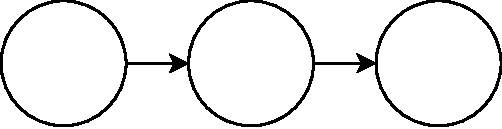
\includegraphics[width=.35\textwidth]{img/graph.pdf}
\end{figure}

\end{frame}

%------------------------------------------------

\begin{frame}[t]{Transformação de dados}

\begin{itemize}
\item \alert{consome} conjuntos de dados (entrada)
\item \alert{produz} conjuntos de dados (saída)
\item corresponde a um ou mais \alert{programas} de simulação
\end{itemize}

\vfill

\begin{figure}
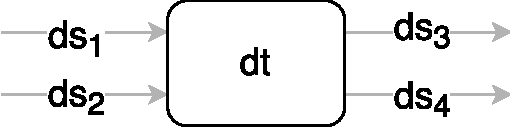
\includegraphics[width=.5\textwidth]{img/example-data-transformation.pdf}
% \caption{Transformação de dados com dois conjuntos de dados de entrada e dois de saída}
\end{figure}

\end{frame}

%------------------------------------------------

\begin{frame}[t]{Conjunto de dados}

\centerline{$ds = (A, C)$}

$\left\{
\begin{tabular}{p{\textwidth}}
\begin{itemize}
    \item \( A = \{da_1, da_2, \ldots, da_{\delta} \} \) : \alert{atributos} de dados
    \item \( C = \{dc_1, dc_2, \ldots, dc_{\zeta} \} \) : \alert{coleções} de dados
\end{itemize}
\end{tabular}
\right.$

\vfill

\begin{figure}
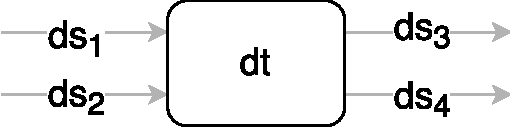
\includegraphics[width=.5\textwidth]{img/example-data-transformation.pdf}
% \caption{Transformação de dados com dois conjuntos de dados de entrada e dois de saída}
\end{figure}

\end{frame}

%------------------------------------------------

{\nologo
\begin{frame}{Atributo de dados}

\centerline{\( A = \{da_1, da_2, \ldots, da_{\delta} \} \)}

$\left\{
\begin{tabular}{p{\textwidth}}
\begin{itemize}
\item $\textup{da} = (\textup{nome},\textup{tipo})$
\item $\textup{\alert{tipo}} \in \{\textup{\small inteiro, ponto flutuante, texto, arquivo, booleano}\}$
\end{itemize}
\end{tabular}
\right.$

\vfill

\begin{exampleblock}{Exemplo}
\begin{table}[htb]
    \centering
    \begin{tabular}{|c|c|}
        \hline
        \textbf{Nome do atributo} & \textbf{Tipo do atributo} \\
        \hline
        Nome             & texto           \\
        \hline
        Idade            & inteiro         \\
        \hline
        Altura \( (m) \) & ponto flutuante \\
        \hline
    \end{tabular}
\end{table}
\end{exampleblock}

\end{frame}
}

%------------------------------------------------

\begin{frame}{Coleção e elemento de dados}

\begin{block}{Coleção de dados}
\begin{itemize}
\item $dc = \{ de_1, de_2, \ldots, de_{\eta} \}$ : \alert{elementos} de dados
\end{itemize}
\end{block}

\begin{block}{Elemento de dados}
\begin{itemize}
\item $de = \{ v_1, v_2, \ldots, v_{\theta} \} \mid \#(ds.A) = \#(de)$ : valores
\end{itemize}
\end{block}

\vfill

\begin{table}[htb]
    \centering
    \begin{tabular}{c|c|c|cc}
        & \textbf{Nome} & \textbf{Idade} & \textbf{Altura \((m)\)} \\
        \( de_{1} \) & Alice   & 22 & \( 1,77 \) & \rdelim\}{2}{.1mm}[\( dc_{1} \)] \\
        \( de_{2} \) & Bob     & 25 & \( 1,79 \) \\
        \( de_{3} \) & Charlie & 42 & \( 1,85 \) & \rdelim\}{1}{.1mm}[\( dc_{2} \)] \\
    \end{tabular}
    \caption{Diferença entre coleção de dados e elemento de dados: \( dc_{1} = \{de_{1}, de_{2}\} \) e \( dc_{2} = \{ de_{3} \} \)}
\end{table}

\end{frame}

%------------------------------------------------

\begin{frame}{Dados de proveniência}

\centerline{$\approx$ \textsc{causalidade}}

\begin{exampleblock}{Proveniência}
\textit{``Lugar de onde alguém ou alguma coisa provém; origem; fonte.''} \\
\hspace*{\fill}--- Dicionário Aulete
\end{exampleblock}

\end{block}{Tipos de proveniência}
\begin{description}[retrospectiva]
\item[prospectiva]
\item[retrospectiva]
\end{description}
\end{block}

\end{frame}

%------------------------------------------------

\section{O problema}
\subsection*{}

% Vitor: O importante é enfatizar o rastreio do fluxo de elementos de dados em uma simulação computacional por meio da abstração de fluxo de dados (no nível lógico). Do ponto de vista de implementação, temos que valorizar as junções "automáticas" (a partir da análise do mapeamento de atributos) e a facilidade em desenvolver uma consulta na nossa abordagem. 

% Marta: Apesar de a ARMFUL ser bem abrangente e eficiente em prover
% consultas envolvendo dados de domínio, de proveniência e de
% execução, ela oferece um recurso limitado para o usuário submeter
% consultas dessas três classes. Na verdade, o usuário precisa não
% apenas conhecer a linguagem SQL, mas conhecer bem os
% relacionamentos que permitem a geração dos relacionamentos
% entre múltiplos arquivos de dados.
% Esse trabalho ter por objetivo facilitar essa interação do usuário
% com a elaboração de consultas analíticas ao utilizar a ARMFUL.
% Comment [2]: Antes de falar da
% contribuição, vc poderia dizer que existem
% soluções para gerar código SQL
% automaticamente, citando-as e se possível,
% explicando porque não foram usadas.

\begin{frame}{O problema}
\todox{Descrever o problema a ser resolvido}
\end{frame}

%------------------------------------------------

\begin{frame}{Proposta}
\todox{Citar o objetivo do trabalho, descrever eventuais vantagens que serão buscadas}
\end{frame}

%------------------------------------------------

\section{Desenvolvimento}

\subsection*{Metodologia}
\begin{frame}{Metodologia}
\todox{Físico, lógico, híbrido}
\end{frame}

\subsection*{Implementação}
\begin{frame}{Implementação}
\todox{Como implementei? Java, HashMultimaps, etc}

\begin{itemize}
\item Java 8
\end{itemize}

\end{frame}

%------------------------------------------------

\section{Experimentos}

\subsection*{Simulação computacional utilizada}
\begin{frame}[t]{Simulação computacional utilizada}{Sedimentação de dinâmica de fluidos computacionais}

\vspace{-.45cm}

\only<1>{
\begin{alertblock}{Objetivo}
\begin{itemize}
\item Simular a turbidez e a perturbação de correntes de fluidos computacionais
\item Observar a \textbf{evolução ao longo do \alert{tempo} entre \alert{fluidos} e \alert{sedimentos}}
\end{itemize}
\end{alertblock}

% https://tex.stackexchange.com/questions/94016/how-to-reduce-space-between-image-and-its-caption
\captionsetup[figure]{skip=-5pt}
\begin{figure}
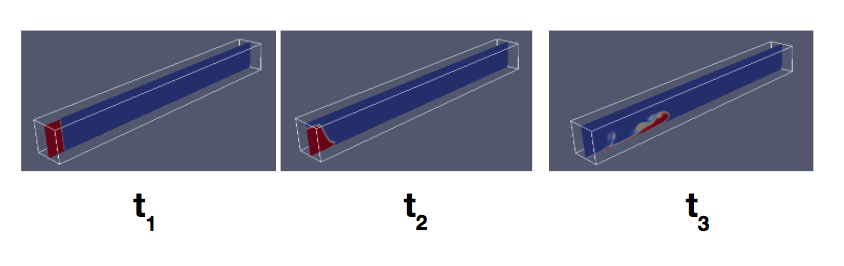
\includegraphics[width=.9\textwidth]{img/sedimentation_over_time.png}\hspace*{\fill}
\caption{Evolução da sedimentação ao longo do tempo}
\end{figure}
}

\only<2>{
\begin{block}{Como?}
\begin{itemize}
\item \texttt{libMesh}: refinamento de malhas e elementos finitos adaptativos
\item equação de incompressibilidade
\item equação de transporte
\end{itemize}
\end{block}

\captionsetup[figure]{skip=-5pt}
\begin{figure}
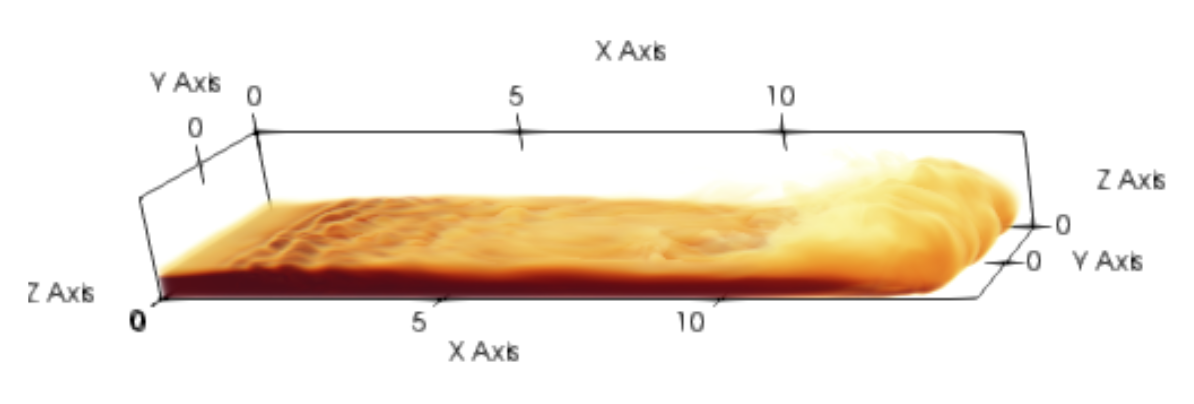
\includegraphics[width=.9\textwidth]{img/sedimentation.png}\hspace*{\fill}
\caption{Ilustração representativa da dinâmica de fluidos}
\end{figure}
}

\note[item]{turbidez encontrada em processos geológicos}
\note[item]{libMesh: biblioteca em C++}
\note[item]{descritos por um modelo matemático que resulta da equação de incompressibilidade de Navier-Stokes (fluido) combinada com uma equação de transporte dominada por advecção (concentração de sedimentos)}
\note[item]{emprega um método de elementos finitos de multi-escala variacional no qual uma abordagem escalonada é utilizada para representar e simular a evolução do tempo nas equações de acoplamento entre o fluido e os sedimentos}
\end{frame}

%------------------------------------------------

\subsection*{Ambiente dos experimentos}
\begin{frame}{Ambiente dos experimentos}

\begin{columns}[t]

\column{.45\textwidth}

\vspace{-.7cm}

\begin{block}{\textit{Solver} de sedimentação}
Execução paralela ($480$~núcleos) no \textit{cluster} Lobo~Carneiro do NACAD\footnotemark{}
\end{block}

\begin{figure}
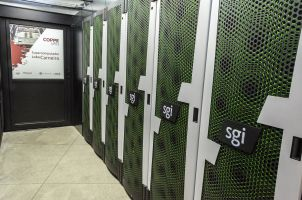
\includegraphics[width=\textwidth]{img/loboc.jpg}
\end{figure}

\setbeamercovered{invisible}
\pause

\column{.45\textwidth}

\vspace{-.7cm}

\begin{block}{Consultas}
Geração e execução em um Macbook Pro Retina 2015:

\begin{itemize}
\item Intel Core i5 2,7~GHz
\item 4~CPUs
\item 8~GB de RAM DDR3
\end{itemize}
\end{block}

\begin{figure}

\includegraphics[width=.75\textwidth]{img/macbook.png}
\end{figure}

\end{columns}

\footnotetext{\url{http://www.nacad.ufrj.br/pt/recursos/sgiicex}}

\end{frame}

%------------------------------------------------

\subsection*{Consultas realizadas}

{\nologo
\begin{frame}{Fluxo de dados utilizado}
\begin{itemize}
\item Fluxo de dados $D^{\prime}$ = ($T^{\prime}$, $S^{\prime}$, $\phi^{\prime}$)
\end{itemize}

\begin{exampleblock}{Alguns atributos de dados de $S^{\prime}$}
\begin{table}[htb]
    \centering
    % https://tex.stackexchange.com/questions/38177/including-large-tables-in-a-beamer-frame
    \resizebox{\linewidth}{!}{% Resize table to fit within \linewidth horizontally
    \begin{tabular}{c|c|c|c}
\textbf{Conjunto de dados}                  & \textbf{Atributo de dados} & \textbf{Tipo}   & \makecell{\textbf{Exemplo} \\ \textbf{de Valor}}             \\ \hline
\multirow{3}{*}{osolversimulationtransport} & time                       & \makecell{ponto \\ flutuante} & $\dfrac{1}{10^5}$                                  \\ \cline{2-4}
                                            & t\_step                    & inteiro         & 0                                      \\ \cline{2-4}
                                            & meshwriter\_task\_id       & inteiro         & 17                                     \\ \hline
\multirow{2}{*}{omeshaggregator}            & xdmf                       & arquivo         & \texttt{$\sim$/output\_48.xmf}             \\ \cline{2-4}
                                            & n\_processors              & inteiro         & 480                                    \\ \hline
omeshrefinement                             & first\_step\_refinement    & booleano        & falso                                  \\ \hline
ovisualization                              & png                        & arquivo         & \texttt{$\sim$/image\_99.png} \\ \hline
oinputmesh                                  & mesh\_file                 & arquivo         & \texttt{$\sim$/necker3d.mesh}               \\ \hline
otimestepcontrolconfig                      & model\_name                & string          & PC11                                  
    \end{tabular}}
    \label{tab:experiments-data-attributes}
\end{table}
\end{exampleblock}

\end{frame}
}

%------------------------------------------------

\begin{frame}

\begin{figure}
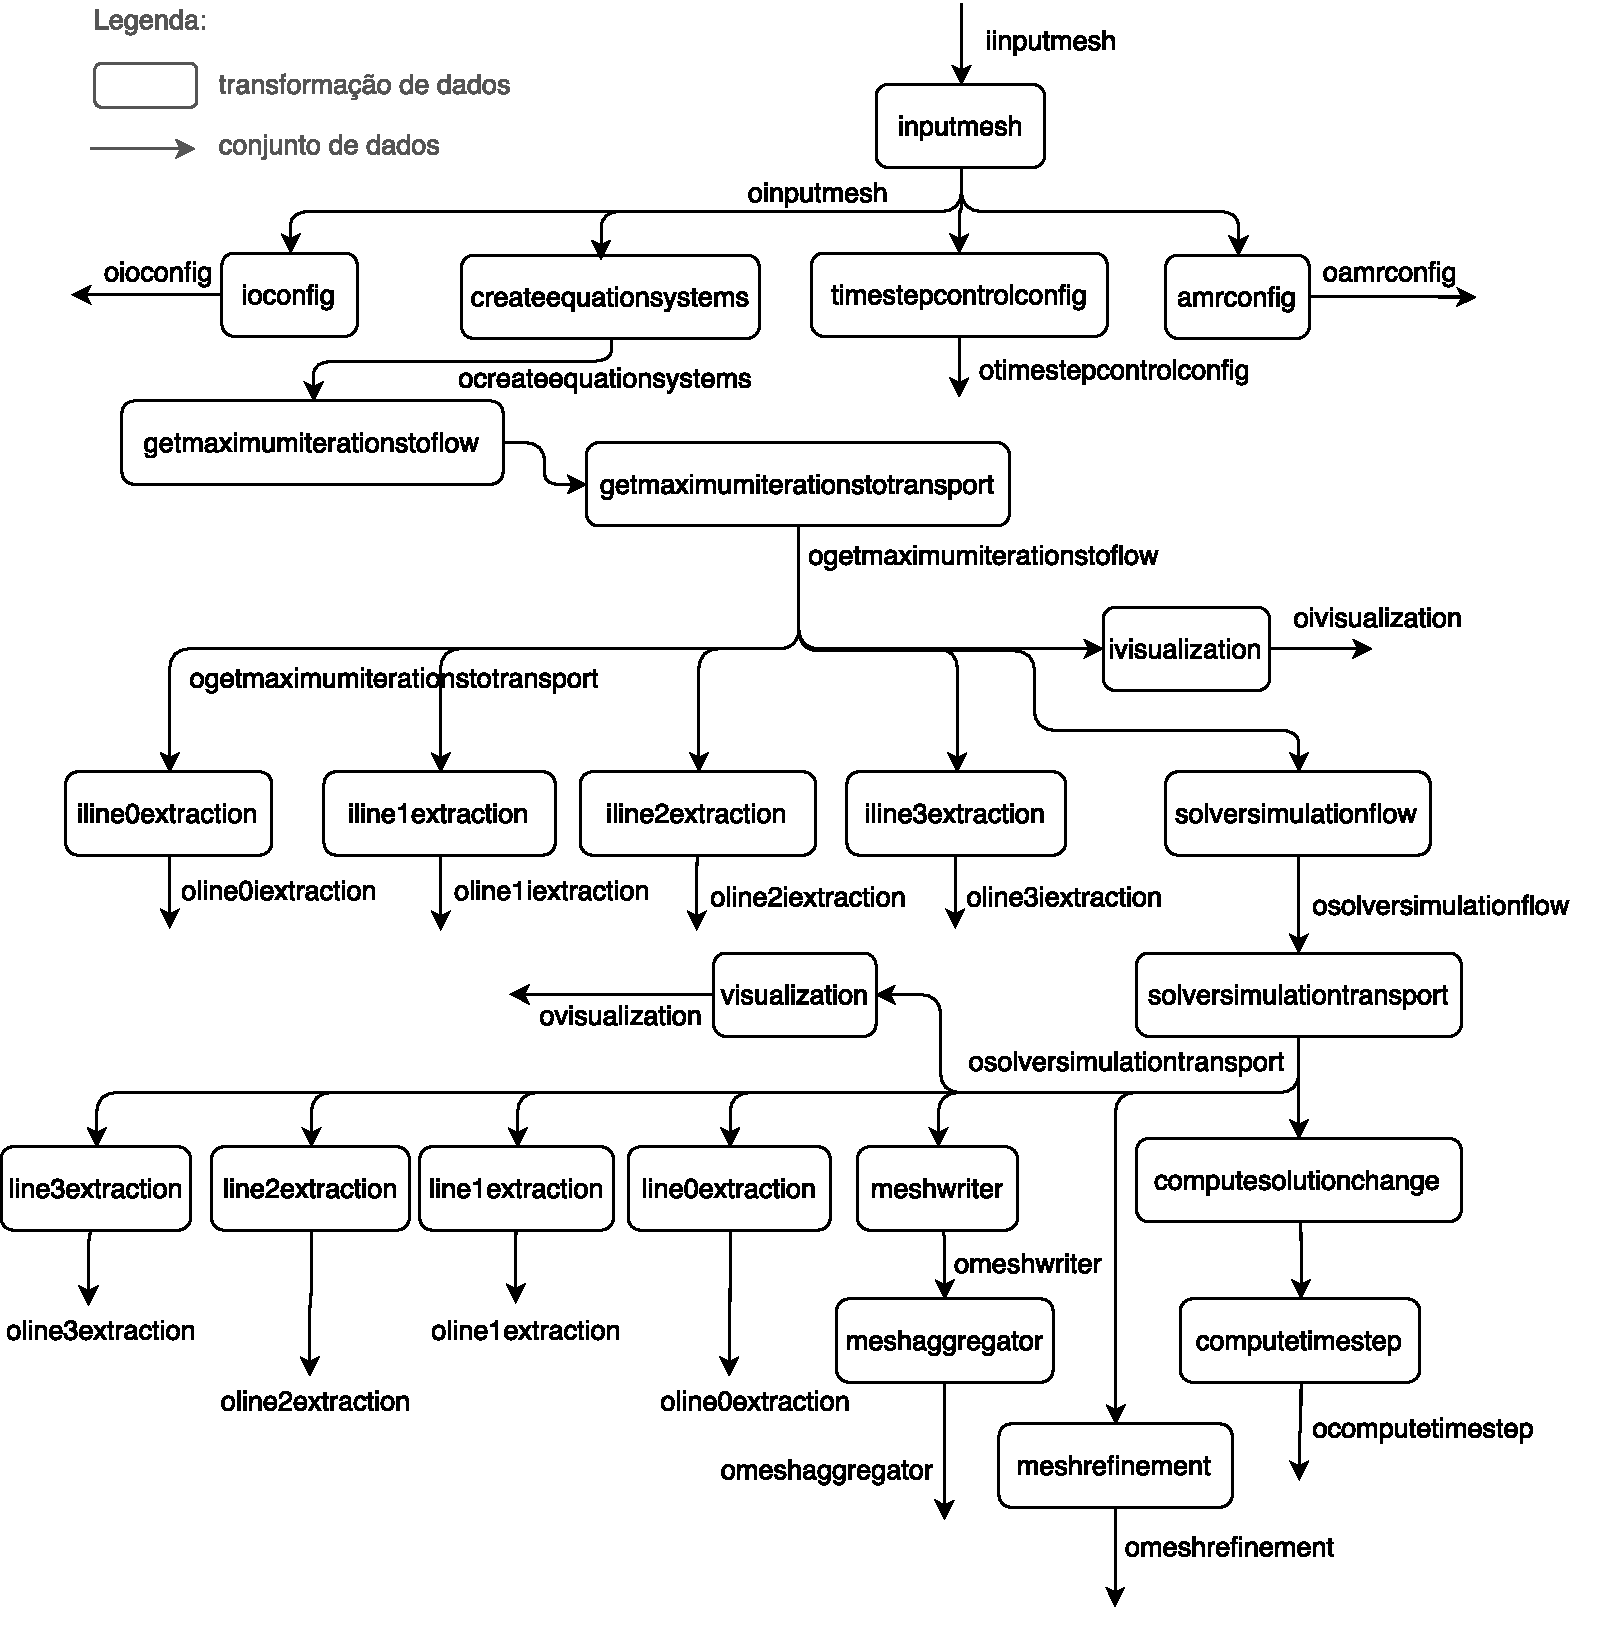
\includegraphics[width=.9\textwidth]{img/slides-dataflow.pdf}
\hspace*{\fill}
\end{figure}

\end{frame}

%------------------------------------------------

{\nologo
\begin{frame}{Consulta \#1}{Especificação}

\begin{block}{Objetivo}
Análise ao longo do \alert{tempo} da média da \alert{concentração de sedimentos} em uma linha extraída de arquivos científicos.
\end{block}

\begin{block}{Argumentos para \texttt{generateSqlQuery}}
\begin{description}[\texttt{dsDestinations}]
\item[\texttt{dsOrigins}] \texttt{osolversimulationtransport}
\item[\texttt{dsDestinations}] \texttt{oline2extraction}, \texttt{omeshwriter}
\item[\texttt{type}] physical
\item[\texttt{projections}] \texttt{osolversimulationtransport.time}, \\ \texttt{AVG(oline2extraction.d)}
\item[\texttt{selections}] $\varnothing$
\end{description}
\end{block}

\end{frame}
}

%------------------------------------------------

{\nologo
\begin{frame}{Consulta \#1}{Elementos mapeados no fluxo de dados}
\begin{figure}
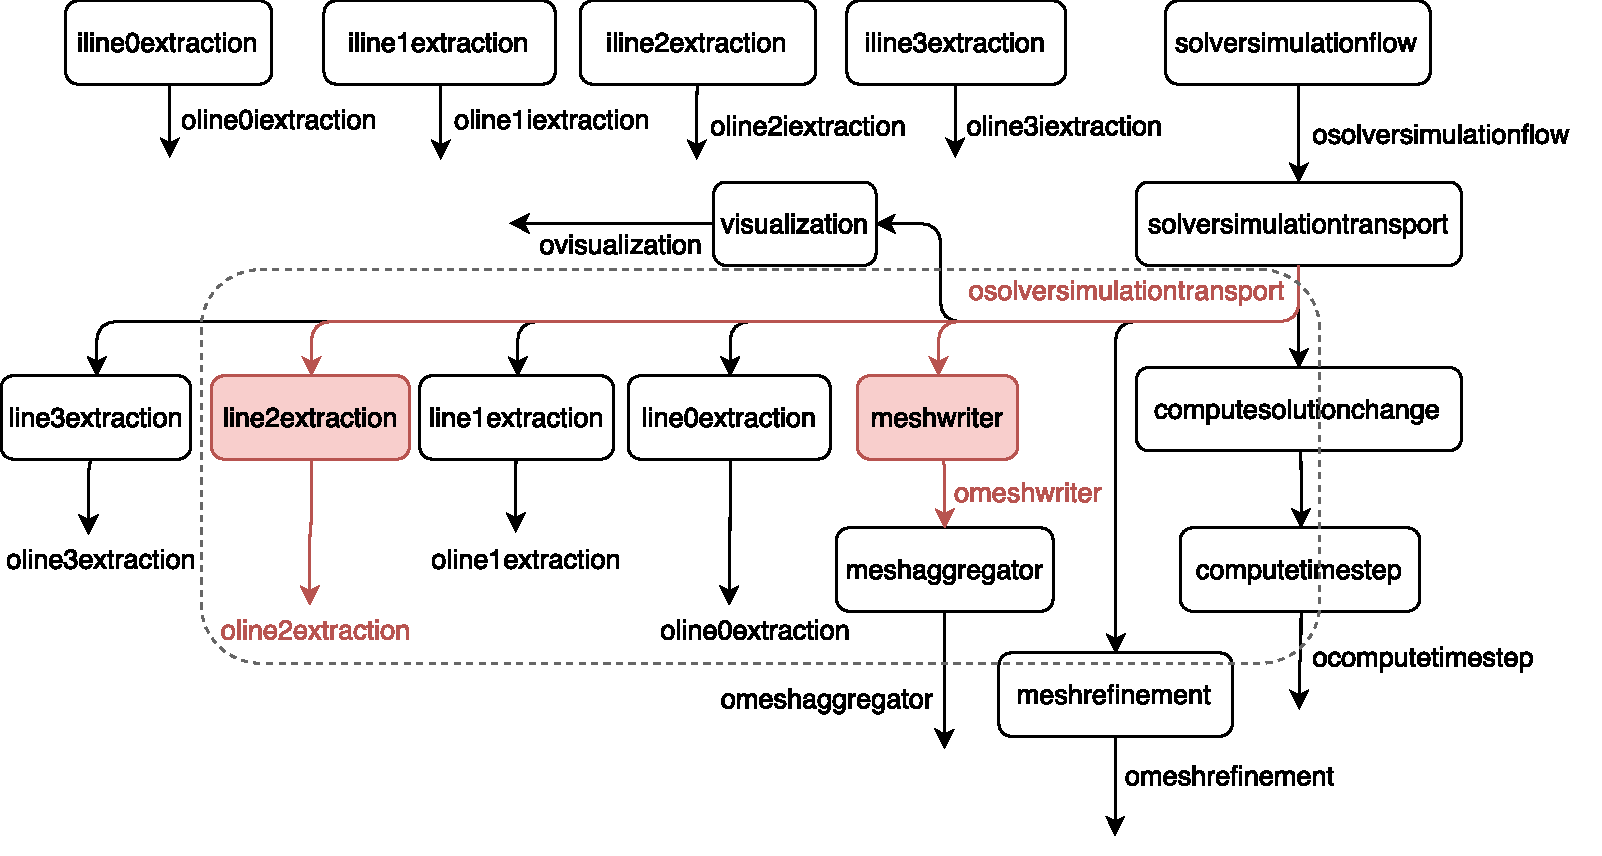
\includegraphics[width=\textwidth]{img/slides-dataflow-1.pdf}
\hspace*{\fill}
\end{figure}
\end{frame}
}

%------------------------------------------------

\begin{frame}[fragile]{Consulta \#1}{SQL gerado}

\begin{lstlisting}[language=sql,deletendkeywords={TIME},caption={tempo médio: 40,29~ms}]
SELECT osolversimulationtransport.time, AVG(oline2extraction.d)
FROM osolversimulationtransport, oline2extraction, omeshwriter
WHERE (osolversimulationtransport.line2extraction_task_id = oline2extraction.line2extraction_task_id) 
AND (osolversimulationtransport.meshwriter_task_id = omeshwriter.meshwriter_task_id)
GROUP BY osolversimulationtransport.time;
\end{lstlisting}

\end{frame}

%------------------------------------------------

\begin{frame}[fragile]{Consulta \#1}{Resultados da consulta SQL}

\begin{center}
\begin{lstlisting}[language=sqlresults,caption={7 tuplas, tempo médio: 4,35~ms}]
+-------------+--------------------------+
| time        | AVG(oline2extraction.d)  |
+=============+==========================+
|   1.3398483 |     1.74129306930693e-44 |
|   3.1009347 |  -1.0847045643564339e-44 |
|   5.4124618 |    7.853749801980205e-39 |
|   7.8695609 |  -1.8180726336633645e-33 |
|  10.1307669 |   1.0729463267326738e-27 |
|  12.6055519 |   1.0473414950495052e-24 |
|          15 |   -8.768540693069305e-22 |
+-------------+--------------------------+
\end{lstlisting}
\end{center}

\end{frame}

%------------------------------------------------

{\nologo
\begin{frame}{Consulta \#2}{Especificação}

\begin{block}{Objetivo}
\small{Análise da concentração de sedimentos em uma linha considerando um instante de tempo fixo e um intervalo específico de valores.}
\end{block}

\begin{block}{Argumentos para \texttt{generateSqlQuery}}
\footnotesize
\begin{description}[\texttt{dsDestinations }]
\small
\setlength\tabcolsep{1.5pt}
\item[\texttt{dsOrigins}] \texttt{osolversimulationtransport}
\item[\texttt{dsDestinations}] \texttt{oline0extraction}, \texttt{omeshwriter}
\item[\texttt{type}] physical
\item[\texttt{projections}] \makecell[l]{\texttt{osolversimulationtransporte.time}, \\ \texttt{oline0extraction.points\{0,1,2\}}, \\ \texttt{oline0extraction.d}}
\item[\texttt{selections}] \makecell[l]{\texttt{osolversimulationtransport.time < 5.5}, \\ \texttt{oline0extraction.d > 0.1}}
\end{description}
\end{block}

\end{frame}
}

%------------------------------------------------

{\nologo
\begin{frame}{Consulta \#2}{Elementos mapeados no fluxo de dados}
\begin{figure}
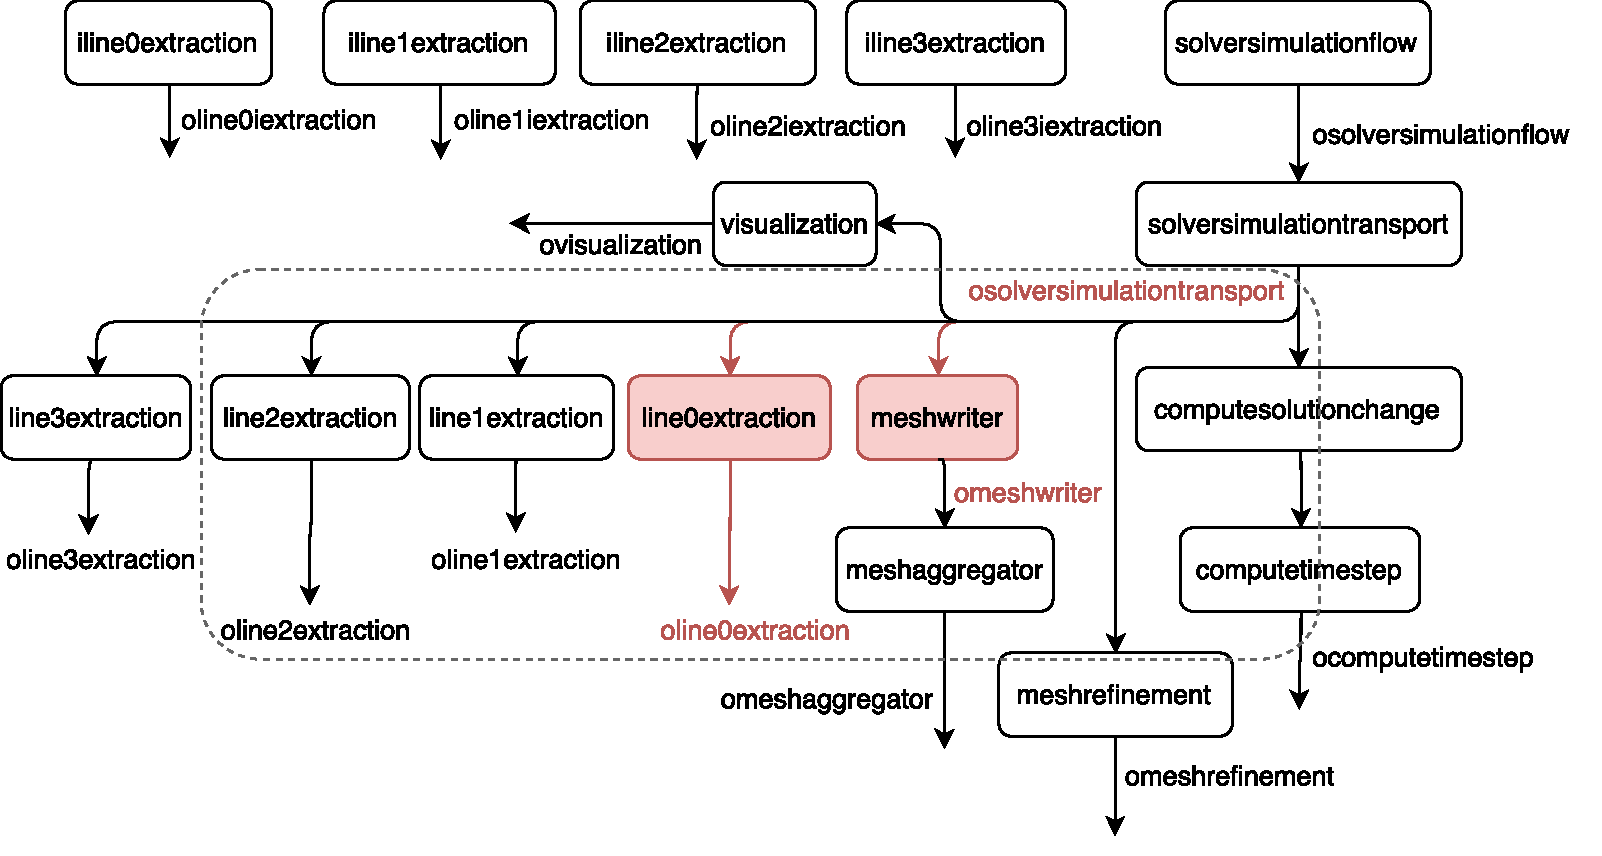
\includegraphics[width=\textwidth]{img/slides-dataflow-2.pdf}
\hspace*{\fill}
\end{figure}
\end{frame}
}

%------------------------------------------------

\begin{frame}[fragile]{Consulta \#2}{SQL gerado}

\vspace{-1.5cm}

\begin{lstlisting}[language=sql,deletendkeywords={TIME},caption={tempo médio: 15,45~ms}]
SELECT osolversimulationtransport.time, oline0extraction.points0, oline0extraction.points1, oline0extraction.points2, oline0extraction.d
FROM osolversimulationtransport, oline0extraction, omeshwriter
WHERE (osolversimulationtransport.time < 5.5) 
AND (oline0extraction.d > 0.1) 
AND (osolversimulationtransport.line0extraction_task_id = oline0extraction.line0extraction_task_id) 
AND (osolversimulationtransport.meshwriter_task_id = omeshwriter.meshwriter_task_id)
LIMIT 10;
\end{lstlisting}

\end{frame}

%------------------------------------------------

\subsection{Resultados}
\begin{frame}{Resultados}
\todox{Tempo, Resultados esperados foram obtidos?, imagens, gráficos, diagramas}
\end{frame}

%------------------------------------------------

\section{Conclusão}

\subsection{Trabalhos futuros}
\begin{frame}{Trabalhos futuros}
\begin{itemize}[<+->]
  \item interface gráfica (visualizador)
  \vfill
  \item validação das especificações do usuário
  \vfill
  \item permitir subconsultas
  \vfill
  \item suportar mais cláusulas SQL:
    \begin{itemize}[<.->]
      \item agregados, \textit{e.g.} \texttt{COUNT(*)} e \texttt{GROUP BY}
      \item \texttt{SELECT DISTINCT}
      \item \texttt{LIMIT}
    \end{itemize}
  \vfill
  \item publicar um \emph{paper}~(!)
\end{itemize}

\note[item]{visualizador: Débora, em andamento. Boa usabilidade. Mouse.}
\note[item]{validação: garantir que conjuntos de dados, atributos de dados, e etc. existam; detectar erros; sintática e semanticamente.}
\note[item]{nome da conferência para o \emph{paper}: VLDB (VERY LARGE DATA BASES) 2018 \url{http://vldb2018.lncc.br/call-for-demostrations.html}}
\end{frame}

%------------------------------------------------

\subsection*{Considerações finais}

{\nologo
\begin{frame}{Considerações finais}{Recapitulando...}

\begin{block}{Simulações computacionais}
\begin{itemize}
\item Fluxo, conjuntos, transformações de dados\ldots{}
\item Mapeamentos de atributos (físico, lógico, híbrido)
\item Dados de proveniência (prospectiva, retrospectiva)
\end{itemize}
\end{block}

\todox{Reiterar o problema / a motivação do trabalho}

\vfill
\pause

\begin{alertblock}{Pré-processador de consultas (QPP)}
\begin{itemize}
\item Arquitetura ARMFUL $\Longrightarrow$ DfAnalyzer $\Longrightarrow$ QPP
\item Análise de dados de domínio, junções automáticas
\item Não há necessidade de se conhecer o esquema do BD
\item Curva de aprendizado, usabilidade
\item \textit{Overhead} de execução pequeno
\end{itemize}
\end{alertblock}

\note[item]{recapitular o conteúdo conceitual abordado}
\note[item]{enfatizar as vantagens do QPP}
\note[item]{defender o propósito do trabalho}
\end{frame}
}

%------------------------------------------------

\begin{frame}{Obrigado!}
\Huge{\centerline{Perguntas?}}

\note[item]{agradecer a atenção das pessoas}
\note[item]{se alguém quiser comentar algo, fique à vontade}
\end{frame}

%------------------------------------------------

% https://tex.stackexchange.com/questions/30461/beamer-nonumber-equivalent-for-slides
\appendix

{
\setbeamertemplate{footline}{}
\begin{withoutheadline}
\begin{frame}{Referências}
\footnotesize{
\begin{thebibliography}{99} % Beamer does not support BibTeX so references must be inserted manually as below

\bibitem[Silva, 2017]{p1} Vítor Silva, Marta Mattoso, Daniel Oliveira et al (2017)
\newblock Raw data queries during data-intensive parallel workflow execution
\newblock \emph{Future Generation Computer Systems}

\bibitem[Silva, 2016]{p1} Vítor Silva, Marta Mattoso, Daniel Oliveira et al (2016)
\newblock In Situ Data Steering on Sedimentation Simulation with Provenance Data
\newblock \emph{SC: High Performance Computing, Networking, Storage and Analysis}

\bibitem[Silva, 2015]{p1} Vítor Silva, Marta Mattoso, Daniel Oliveira et al (2015)
\newblock Analyzing related raw data files through dataflows
\newblock \emph{Concurrency and Computation: Practice and Experience}

\end{thebibliography}
}
\end{frame}
\end{withoutheadline}
}

%------------------------------------------------

{
\setbeamertemplate{footline}{}
\begin{frame}{Slides}
Disponíveis em: \url{https://speakerdeck.com/thiagowfx}
\end{frame}
}

%------------------------------------------------

% \begin{frame}
% \frametitle{Table}
% \begin{table}
% \begin{tabular}{l l l}
% \toprule
% \textbf{Treatments} & \textbf{Response 1} & \textbf{Response 2}\\
% \midrule
% Treatment 1 & 0.0003262 & 0.562 \\
% Treatment 2 & 0.0015681 & 0.910 \\
% Treatment 3 & 0.0009271 & 0.296 \\
% \bottomrule
% \end{tabular}
% \caption{Table caption}
% \end{table}
% \end{frame}

%------------------------------------------------

% \begin{frame}
% \frametitle{Figure}
% Uncomment the code on this slide to include your own image from the same directory as the template .TeX file.
%\begin{figure}
%\includegraphics[width=0.8\linewidth]{test}
%\end{figure}
% \end{frame}

%----------------------------------------------------------------------------------------

\end{document}